% =====================================================================
%  PHỤ LỤC E. POSTER VÀ STANDEE
%  Poster theo mẫu BM07A: in màu 1 bản A1 (báo cáo triển lãm) và 1 bản A3
%  (đóng vào cuốn báo cáo tổng kết). Standee theo mẫu BM07B.
% =====================================================================
\chapter{Poster và standee của đề tài}
\label{pl:e}

Poster của đề tài được trình bày theo mẫu BM07A/QT-PKHCN-NCKHSV/00: khổ A3 nằm ngang, bốn cột, gồm phần đầu (tên đề tài, mã số, giảng viên hướng dẫn, sinh viên thực hiện, email, khoa, logo trường và logo đơn vị), phần tóm tắt kèm từ khoá, và bốn mục I--IV cùng tài liệu tham khảo. Bản in triển lãm khổ A1 dùng cùng nội dung, phóng theo tỷ lệ 2:1 (tệp \texttt{poster\_a3/poster\_a1.pdf}).

Standee của đề tài (tệp \texttt{standee/standee.pdf}) trình bày theo mẫu BM07B/QT-PKHCN-NCKHSV/00, khổ 0,6 $\times$ 1,6\,m, gồm năm mục I--V.

Trang sau là bản poster khổ A3 đóng kèm theo quy định.
\clearpage
\IfFileExists{../poster_a3/poster_a3.pdf}{%
  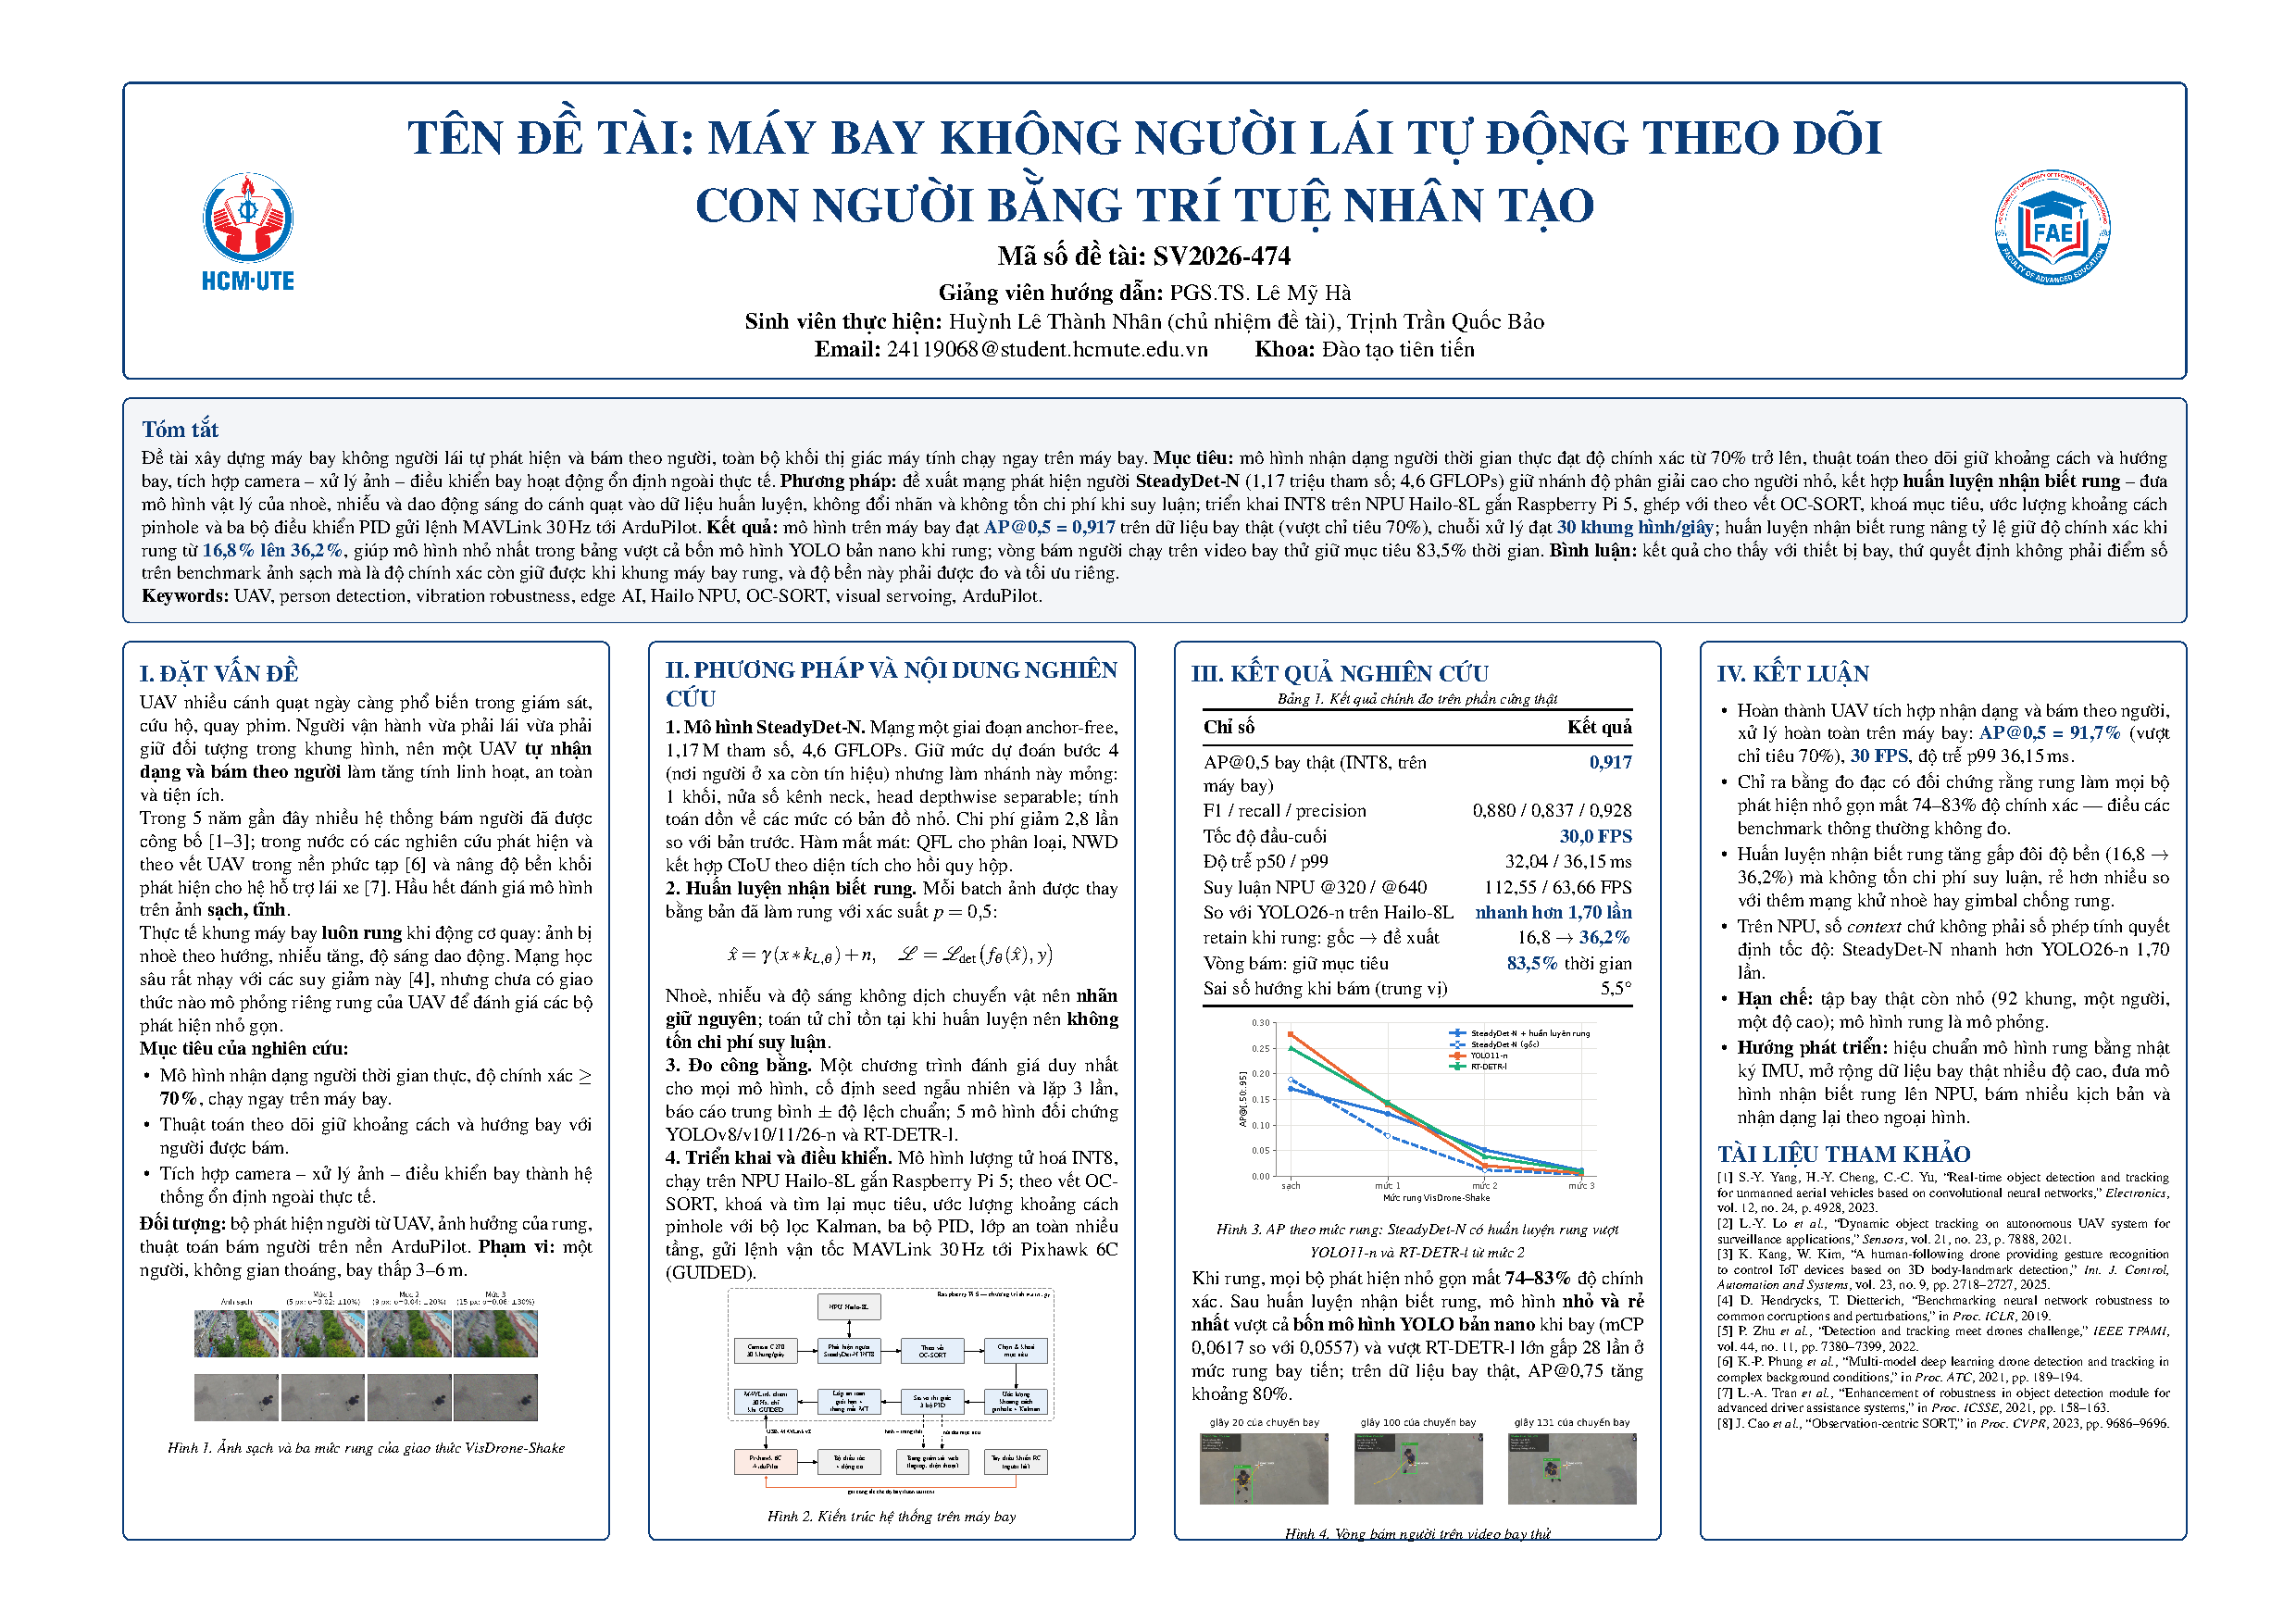
\includepdf[pages=1,angle=90,fitpaper=false,scale=0.68,
              pagecommand={\thispagestyle{empty}}]{../poster_a3/poster_a3.pdf}}{}
